The $\wenuplusjets$ process can pass the signal region selection, thus
contributing to the background, in case the electron is not identified in the
detector; in the $\wtaunuplusjets$ process the $\tau$ particle can decay
hadronically in the 68\% of the cases resulting in additional jets that can
enter the signal region selection even with no ISR\@. This region
(CR$_\mathrm{\, ele}$) contains mainly $\wenuplusjets$ events and is designed to
constrain also $\wtaunuplusjets$ processes and estimate their contribution to
the background in the signal region. In order to increase the rejection of
multi-jet background, the electron is retained in the $\met$ calculation, the
missing transverse momentum in this case resembles more the escaping neutrino
$\pt$. The CR$_\mathrm{\, ele}$ region selects events with:
\begin{itemize}
\item Exactly one good electron.
\item Reject any other good electron.
\end{itemize}
In order to enhance the $\wtaunuplusjets$ contribution in this region, no
$m_\mathrm{\, T}$ cut is applied. Figure~\ref{fig:ele_cr_plots} shows the
measured $\met$ and the leading jet $\pt$ distribution in this control
region. The overall agreement between data and MC is good and improved after the
global likelihood fit procedure described in \cref{sec:glob-simult-likel}.

\begin{figure}[!h]
  \centering
  \begin{subfigure}[t]{.48\linewidth}
    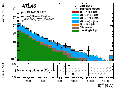
\includegraphics[width=\linewidth]{ele_cr_et_miss_post_fit}
    \caption{$\met$ distribution.}
    \label{fig:ele_cr_et_miss_pre_fit}
  \end{subfigure}
  \begin{subfigure}[t]{.48\linewidth}
    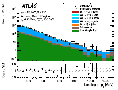
\includegraphics[width=\linewidth]{ele_cr_jet1_pt_post_fit}
    \caption{Leading jet $\pt$ distribution.}
    \label{fig:ele_cr_jet1_pt_pre_fit}
  \end{subfigure}
  \caption{Measured $\met$ and leading jet $\pt$ after fit distribution in the
    electron CR for the $\met > 250~$GeV selection. The error bands include the
    statistical and systematic error.}
  \label{fig:ele_cr_plots}
\end{figure}
%%% Local Variables:
%%% mode: latex
%%% TeX-master: "../search_for_DM_LED_with_ATLAS"
%%% End:
